\chapter{Discussion}
This section presents a summary of the significant factors in designing good models, outlining the advantages and disadvantages; implications of the empirical results for deploying fall detection systems in practice; and limitations and future research.

\section{Significant Factors in Designing Good Models}

In this research, we discovered the following pros and cons with PoseNet and OpenPose for creating fall detection algorithms. During our research in creating, testing and comparing our two pose detection systems, we found that each have some drawbacks as well as advantages.

Advantages:
\begin{itemize}
    \item PoseNet can be run on mobile devices, low computation power required
    \item PoseNet is free to use commercially
    \item OpenPose has better tracking of people partially obstructed by an object
\end{itemize}

Disadvantages:
\begin{itemize}
    \item Both OpenPose and PoseNet have issues with detecting people where there are none, specifically on black objects like the legs of an office chair, etc.
    \item People falling behind objects is difficult for both OpenPose and PoseNet, though less so for OpenPose. PoseNet will lose tracking entirely with any obstruction, whereas OpenPose is able to better maintain tracking on partially obstructed people.  This is likely due to the number of respective keypoints each system uses for pose estimation.
    \item OpenPose requires high computational power, generally runs on a powerful computer.
    \item OpenPose requires a substantial amount of money for commercial deployment
\end{itemize}


PoseNet ultimately led to the better fall detection results over the OpenPose based system, even though OpenPose’s pose detection is slightly more accurate and richer in data (i.e., number of keypoints). It is not exactly clear why this was the case, but it is hypothesized that when people are falling, and due to their higher acceleration, pose data is more unique for OpenPose to analyze. So, this may make it easier for the OpenPose based machine learning models to differentiate \textit{fall} frames from \textit{non-fall} frames.


Our fall detection system with PoseNet can be run easily on mobile devices as opposed to the system using OpenPose, which requires substantially more computational power. OpenPose requires a powerful computer and simply could not be run on a mobile device at this time. Furthermore, PoseNet, unlike OpenPose, is free to use for any purpose.


Both systems exhibit issues especially when trying to detect falls when a person falls behind an obstacle, like a piece of furniture. Partial obstruction of the image of the person on video frames causes PoseNet to lose tracking entirely, while OpenPose does a somewhat better job of keeping track of the person, but still has issues. Objects in the background in frames also tend to confuse both pose detectors, especially black objects such as the legs of an office chair being confused for the legs of a person (Figure ~\ref{fig:falseidentification} and ~\ref{fig:falseidentification2}). Reflections in mirrors and windows, if vivid enough, can also cause false pose detections with both PoseNet and OpenPose.



\begin{figure}
  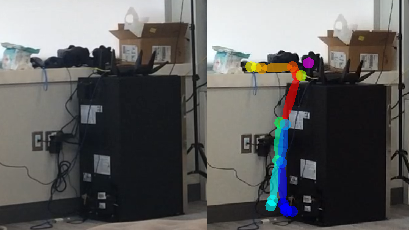
\includegraphics[width=\linewidth]{falseidentification}
  \caption{Frame from the video containing a collection of cables that strangely resemble a person (left), false identification of a person (right).}
  \label{fig:falseidentification}
\end{figure}




The addition of a frame history ML model analyzing the output data of the frame-by-frame data model proved to increase accuracy early on in the research that we conducted and seems to be a step in the right direction for improving fall detection based on pose analysis. The optimum size of the frame history to be analyzed has yet to be determined.  While 25 and 30 frame size histories were used in our models with PoseNet and OpenPose respectively that produced good results, further experimentation should be done to determine the optimal number of frames that should be kept track of for the sake of the most accurate fall detections. Frame history was taken into consideration in this study based on the idea that a fall cannot truly be expressed in one frame in isolation from video footage. At any given frame, it is difficult to tell for sure if one is falling, or is just performing an activity of daily living (e.g., crouching, bending down, lying down, etc.). With the ability for the ML model to look through predictions based on video frames in the past, we aim to capture the moment of the person standing, starting to fall, and landing on the ground in a collapsed position.


In our experiments, we filmed participants in a variety of falling and non-falling scenarios. This brought a great deal of diversity into the dataset but was not without fault. No actual elderly people like the ones this research was targeted at helping were involved in the videos filmed, and the dataset contained far too many non-falling states in comparison to the number of falling states in frames in the videos. Had the video data been carefully cut down to show only the moment of falling from start to finish, with no extra non-falling data of any kind, perhaps the results would have shown a more balanced distribution of fall state and non-fall states. Furthermore, our dataset is arguably small – more videos of moments of people falling may improve the training processes. It is not clear whether it would help, but introducing more scenarios of activities of daily living may increase the accuracy of our models, such as having people carrying things (e.g., drinking glasses, plates), or lying down in a bed, etc.

\begin{figure}
  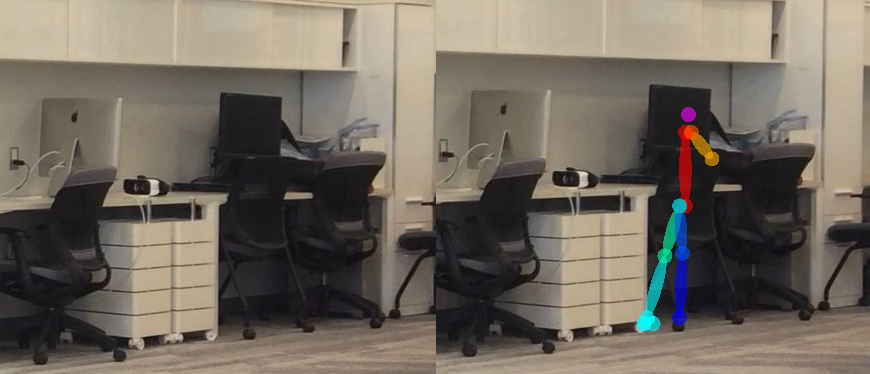
\includegraphics[width=\linewidth]{falseidentification2}
  \caption{Wheels and bottom structure of an office chair mistakenly identified as a person’s leg.}
  \label{fig:falseidentification2}
\end{figure}



\section{Implications for Practice}

Multiple camera feeds into our algorithm would facilitate more comprehensive coverage of the person’s environment and increase the overall accuracy of our system and the confidence of detecting a fall especially in these types of situations.

\section{Limitations}

This research showed that there is significant potential to create classifiers using machine learning to determine if a person has fallen or not. As with any research there are limitations. Some of the main limitations of this work are presented below.

\subsection{Sensitivity}

The lower than desired sensitivity values in both fall detection systems implies that our experimental data did not contain enough frames where participants were actually falling for the machine learning models to truly learn when falls should be detected at all times. This is evident when one compares the total true positive plus false negative portion to the total true negative plus false positive portion in Tables 1 and 2. There are significantly more non-fall frame data in comparison to fall frame data. Almost all videos predictably contained 90\%+ frames where people were not in the middle of a fall, and that was likely the reason for this outcome.


\subsection{Computational Power}

The computational power required for the OpenPose based fall detection system was much higher than that needed for the PoseNet based solution. The PoseNet system has been optimized to work even on mobile devices whereas OpenPose requires a powerful system. To use a fall system based on OpenPose in practice would likely prove to be much more expensive to run than one that is based on PoseNet. This is especially a problem if one is trying to run the fall detection system in real time on a live camera feed. Running pose detection in OpenPose typically requires slowing down the video to compensate for the work the computer needs to do.

The number of participants involved in this study was sufficient for exploring how these pose detection fall prediction systems might be implemented and for discovering ways to improve upon them. However, having a much larger video dataset of say, 100 or even a 1,000 people, would likely enhance the machine learning models featured here.

\subsection{False Detections}
Even with the more sophisticated pose detection tool, OpenPose, as well as with PoseNet, there were plenty of false detections of human poses such as in background objects in the videos filmed in this research. As can be seen in Figure ~\ref{fig:falseidentification} for example, a fridge and a mix of cables was detected as a person by OpenPose, and in Figure ~\ref{fig:falseidentification2}, a chair next to a computer monitor was detected as another person. This would also happen with any detailed reflections in videos, if there were any on windows or mirrors, and at some points, people were falsely detected to be sitting on a couch in the background when no one was there at all. These false pose identifications in video frames throughout the datasets tested on can of course lead to worse results when fed to a machine learning model that will try to learn partially based off of the false information.


In this study, a single-pose version of PoseNet was used, and a multi-person version of OpenPose. These seemed to work best for what we were trying to study at the time, but it is possible that with further examination of other possible versions of the PoseNet/OpenPose algorithms, new results could be found. OpenPose could be configured to detect only one person in a frame, or PoseNet could be configured to detect multiple. It is likely however, that if PoseNet is configured for multiple person detection, the system would require more computational power, but it is unlikely to be as much as what OpenPose requires.

